\subsection{Differenze tra Gradle e Maven} % https://gradle.org/maven-vs-gradle/
Ci sono molte differenze tra questi due tools: flessibilità, performance, gestione delle dipendenze e molto altro. La configurazione di Gradle in un progetto ha una convenzione molto più facile e comprensibile rispetto alla tediosa e a volte impossibile configurazione del pom.xml di Maven, anche se entrambi usano dei metodi di miglioramento della velocità di esecuzione delle build. Grandle usufruisce di:
\begin{itemize}
    \item \textbf{Incrementality:} evitando il lavoro di monitoraggio dei task di I/O eseguendo solo il necessario e quando possibile processare solo i files che sono cambiati;
    \item \textbf{Build Cache:} utilizza un sistema di cache riusando gli outputs di altre build Gradle con gli stessi inputs;
    \item \textbf{Deamon:} sfrutta un long-lived process che mantiene tutte le informazioni in memoria.
\end{itemize}
Queste 3 caratteristiche rendono Gradle molto veloce, ad esempio una build Gradle con Maven verrebbe completata con un tempo 3 volte maggiore. Tutto questo è anche possibile grazie a un sistema di esecuzioni parallele di task e intra-task.
\begin{figure}[H]
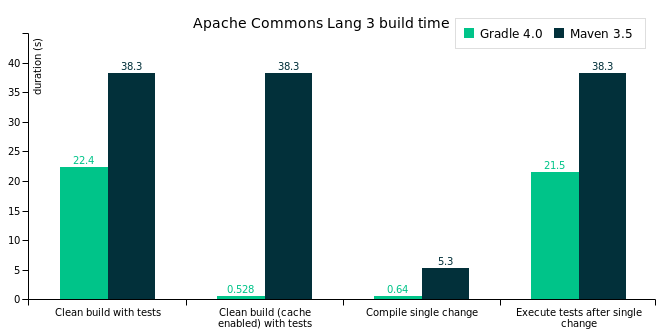
\includegraphics[scale=0.70]{introduction/subsection/gradle/performance.png}
\end{figure} 
% https://docs.gradle.org/current/userguide/userguide.html
